%%% 2022年 7月30日 星期六 10时49分17秒 CST
%%% author: 李小丹(Shao-Dan Lee) 字 殊恒(Shuheng)

\usepackage[utf8]{inputenc}
\usepackage{latexsym}
\usepackage{textcomp}
\usepackage[no-math]{fontspec}
\usepackage[defaultfam,tabular,lining,scaled=1.02]{montserrat}
\usepackage[varqu,varl]{zi4} % sans serif typewriter
% \usepackage[scaled=1.1]{newtxsf} %or stix2
% \usepackage[defaultmathsizes,italic]{mathastext}
\usepackage{expl3}
% \usepackage{makeidx}
% \usepackage{verbatim}
% \usepackage[runin]{abstract}
\usepackage[margin=2cm,hmarginratio=1:1]{geometry}
\usepackage{graphicx}
% \usepackage[svgnames,table]{xcolor}
\usepackage[svgnames]{xcolor}
\usepackage{tikz}
\usepackage{lilyglyphs}
\usepackage[most]{tcolorbox}
\usepackage{multicol}
% The package "background" is not good,
% may use tikz or eso-pic
% cf. https://tex.stackexchange.com/questions/167719/how-to-use-background-image-in-latex
\usepackage[some]{background}
\usepackage{soul}
%\usepackage{emoji}
\usepackage[fixed]{fontawesome5}
% \usepackage{byo-twemojis}
\usepackage{twemojis}
% \usepackage{ulem}
\usepackage{enumitem}
\usepackage{calc}
% \usepackage{ifthen}
% \usepackage[center]{titlesec}
\usepackage[calcwidth]{titlesec}
\usepackage{tocdata}
%\usepackage{tocloft}
\usepackage{fancyhdr}
\usepackage{multirow}
\usepackage{longtable}
\usepackage{tabu}
\usepackage{multirow}
\usepackage{pgfornament}
% \usepackage{qrcode}
%%% cf. https://github.com/EagleoutIce/fancyqr/
\usepackage{fancyqr}
\usepackage{changelog}
\usepackage{xeCJK}
\usepackage[fontset=macnew]{ctex}

\makeatletter


\newcommand{\mytitle}{乐谱集}
\newcommand{\myname}{Shao-Dan Lee}
\newcommand{\mycnname}{李小丹\ 编著}
\newcommand{\myemail}{leeshuheng@icloud.com}

\author{\mycnname}
\title{\mytitle}
%\email{\myemail}
\date{\today}

\usepackage[bookmarks, pdfpagelabels, colorlinks]{hyperref}

% \usepackage{amsrefs}
\usepackage{bookmark}
\usepackage[noabbrev]{cleveref}
% polyglossia package should be last loaded.
\usepackage{polyglossia}

\usetikzlibrary{graphs}
\usetikzlibrary{shapes.misc}
\usetikzlibrary {shapes.callouts}
\usetikzlibrary{shadows}
\usetikzlibrary{chains}
\usepgflibrary {shadings}

\hypersetup {
	pdftitle={\mytitle},
	pdfsubject={Music score},
	pdfauthor={李小丹},
	pdfcreator={李小丹},
	%citecolor = MediumVioletRed,
	% citecolor = DarkViolet,
	citecolor = BlueViolet,
	linkcolor = RoyalBlue,
	%urlcolor = SeaGreen
	urlcolor = DarkTurquoise
}

%% from %%%
%% https://tug.org/pipermail/xetex/2008-December/011420.html
% \newfontfamily\semibf{FiraSans SemiBold}
%% https://tex.stackexchange.com/questions/536367/how-do-i-use-light-normal-semibold-and-bold-font-types-in-one-document-using
% \newcommand{\mynotation}{\textbf{\sourcesansprolight\underline{Notation}}}
% \newcommand{\mynotation}{\firasemibold\underline{Notation}}
\newcommand{\mynotation}{\fontseries{semibold}\selectfont Notation}
% \newcommand{\mynotation}{\fontseries{semibold}\selectfont\underline{Notation}}

% \renewcommand{\thefootnote}{\fnsymbol{footnote}}
% \renewcommand{\thefootnote}{\alph{footnote}}

% \renewcommand{\cftsecleader}{\bfseries\cftdotfill{\cftdotsep}}
% \renewcommand{\cftsecleader}{\cftdotfill{\cftdotsep}}

% \ctexset{fontset = macnew}
%\lishu and \youyuan

\def\cclink{https://creativecommons.org/licenses/by/4.0/}
\def\ccby{\href{\cclink}{\faCreativeCommons\faCreativeCommonsBy}}

\backgroundsetup{
	scale=1,
	angle=0,
	opacity=1,
	contents={
		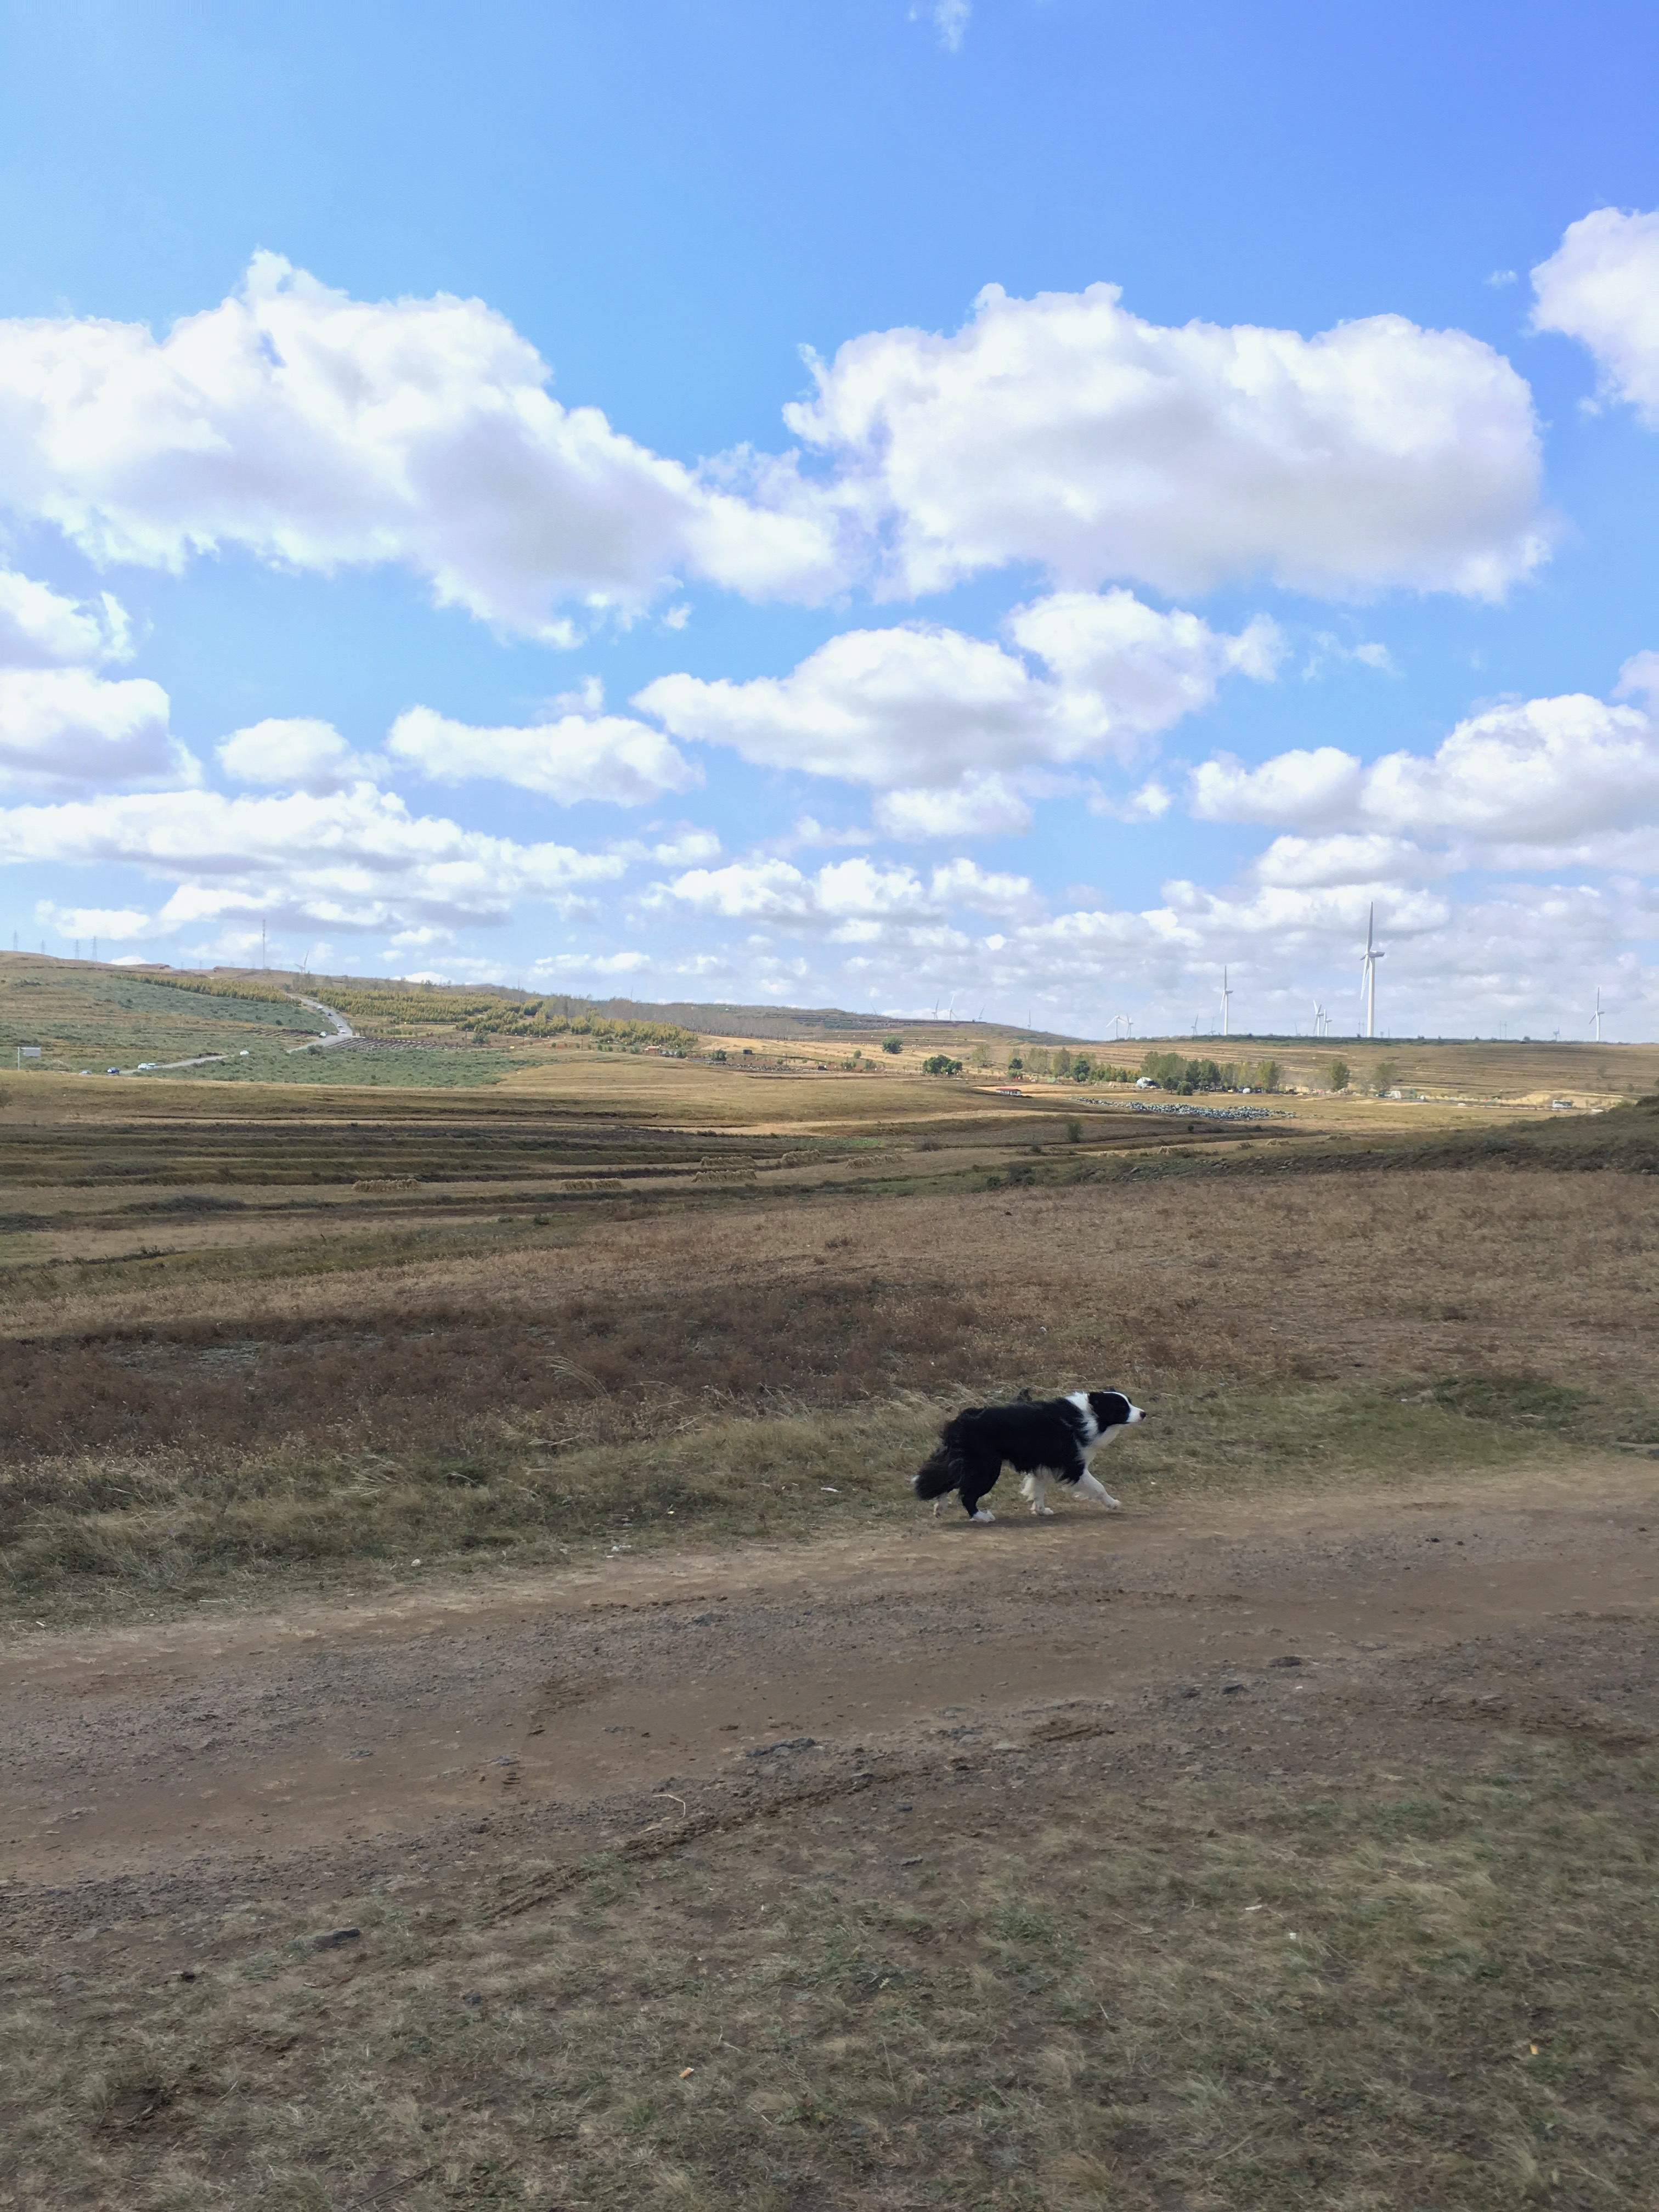
\includegraphics[width=1.00\paperwidth,height=\paperheight]{./alpha.jpeg}
	}
}
%% cf. manual of titlesec
\titleformat{\section}[block]{%
	\filcenter\large%
	\addtolength{\titlewidth}{2pc}%
%	\titleline*[c]{\titlerule*[.6pc]{\textbullet}}%
	\titleline*[c]{\titlerule*[0.6cm]{\lineornament{0.6cm}{0.30cm}{1}{70}}}%
	\addvspace{3pt}%
	\normalfont\bfseries}%
{\thesection}{1em}{}
\titlespacing{\section}{5pc}{*1}{0pt}[5pc]
% \def\fullsection#1#2#3{%
% 	\begin{center}
% 	{\large
% 	\lineornament{0.7cm}{0.3cm}{#3}{70}\\
% 	\phantomsection%
% 	\addcontentsline{toc}{section}{\protect\textbf{#1}}%
% 	{#1}
% 	\markboth{#2}{#1}%
% 	}%
% 	\end{center}
% }

%%% enhanced jigsaw:
%%  cf.~https://tex.stackexchange.com/questions/489714/transparency-option-in-tcolorbox
%%  and manual[10.11 Jigsaw Skin Variants]
%% Don't use \tcbox! Can't use \ht... in tcolorbox
% \newbox\clefhbox
% \setbox\clefhbox=\hbox{{\fontsize{36}{0}\selectfont\clefG}}
\def\clefGbox{
	\begin{tcolorbox}[width=3.5cm, square, circular arc, boxrule=0.5mm,
	       opacityframe=0.5, opacityback=0.3, enhanced jigsaw,
		colframe=MediumSpringGreen, colback=DodgerBlue,
		coltext=DarkViolet, halign=center, valign=center]
			{\fontsize{36}{0}\selectfont\clefG}
	\end{tcolorbox}
}
\def\titlebox#1#2{%
	\begin{tcolorbox}[beamer, width=0.7\hsize, arc=4mm,
		colframe=MediumSpringGreen, colback=DodgerBlue,
		coltext=white, halign=center, valign=center,
		halign lower=center, valign lower=center]
%		#1\\\vskip0.5cm\tcblower #2
		#1\\\vskip0.5cm #2
	\end{tcolorbox}
}
\def\datebox#1{
	\begin{tcolorbox}[arc = 3mm, boxrule=0.5mm, width=0.3\hsize,
	       opacityframe=0.5, opacityback=0.3, enhanced jigsaw,
		colback=MediumSpringGreen, colframe=DodgerBlue,
		coltext=white, halign=center, valign=center]
			#1
	\end{tcolorbox}
}
%% from manual tikz
\def\drawcallout#1#2#3{
\begin{tikzpicture}[remember picture, note/.style={ellipse callout, fill=LightSkyBlue}]
%	\draw [help lines] grid(17,3);
%	\node [note=red!50, callout relative pointer={(0,1)}] at (3,1) {Relative};
%	\node [note=blue!50, callout absolute pointer={(0,1)}] at (1,0) {Absolute};
	\node [draw, note=white, opacity=.5, overlay, callout relative pointer={#1}] at #2 {#3};
\end{tikzpicture}
}
%% copy from manual
\newcommand{\eachpageornament}{%
	\begin{tikzpicture}[remember picture, overlay]
	\node[anchor=north west, color=SlateBlue] at (current page.north west){%
		\pgfornament[width=0.8cm]{61}};
	\node[anchor=north east, color=SlateBlue] at (current page.north east){%
		\pgfornament[width=0.8cm,symmetry=v]{61}};
	\node[anchor=south west, color=SlateBlue] at (current page.south west){%
		\pgfornament[width=0.8cm,symmetry=h]{61}};
	\node[anchor=south east, color=SlateBlue] at (current page.south east){%
		\pgfornament[width=0.8cm,symmetry=c]{61}};
	\end{tikzpicture}%
}%
\newcount\pos
%% cf. manual
\newcommand{\lineornament}[4]{%
\begin{tikzpicture}[start chain,node distance=0,inner sep=0]
%	\node[minimum size=4pt,inner sep=0] (A) at (0,0){};
%	\coordinate (B) at (8,0);
	{%[start chain,node distance=0,inner sep=0]
	\node[anchor=west] [on chain] at (0, 0) {\pgfornament[height=#2,width=#1]{#4}};
%	\node [on chain] {\pgfornament[width=1cm]{70}};
%	\node [on chain] {\pgfornament[width=1cm]{70}};
%	\node [on chain] {\pgfornament[width=1cm]{70}};}
	\count\pos=1
	\loop
		\ifnum \count\pos < #3
			\node [on chain] {\pgfornament[height=#2,width=#1]{#4}};
			\advance\count\pos by 1
	\repeat
	}
\end{tikzpicture}%
}
% from https://tex.stackexchange.com/questions/167719/how-to-use-background-image-in-latex
\long\def\picbackground#1#2{%
\tikz[remember picture,overlay]
	\node[opacity=#2,inner sep=0pt] at (current page.center){%
	\includegraphics[width=\paperwidth,height=\paperheight]{#1}};%
}
% cf. https://tex.stackexchange.com/questions/519676/how-to-make-this-watermark
% https://tex.stackexchange.com/questions/527342/watermark-in-tikz-image
% https://texblog.org/2012/02/17/watermarks-draft-review-approved-confidential/
% https://www.latex4technics.com/?note=1c9f
% To use it,
% for example \awatermark{李小丹}{0.4}{45}{16}{gray}{current page.center}
% \long\def\awatermark#1#2#3#4#5#6{%
% \tikz[remember picture,overlay]
% 	\node[opacity=#2,inner sep=0pt,rotate=#3,scale=#4,color=#5] at (#6){%
% 	#1};%
% }

%% from manual
\definecolor{nicered}{rgb}{.647,.129,.149}
\makeatletter
\newlength\dlf@normtxtw
\setlength\dlf@normtxtw{\textwidth}
\def\myhelvetfont{\def\sfdefault{mdput}}
\newsavebox{\feline@chapter}
\newcommand\feline@chapter@marker[1][4cm]{%
\sbox\feline@chapter{%
	\resizebox{!}{#1}{\fboxsep=1pt%
	\colorbox{nicered}{\color{white}\bfseries\sffamily\thechapter}%
}}%
\rotatebox{90}{%
	\resizebox{%
		\heightof{\usebox{\feline@chapter}}+\depthof{\usebox{\feline@chapter}}}%
	{!}{\scshape\so\@chapapp}}\quad%
\raisebox{\depthof{\usebox{\feline@chapter}}}{\usebox{\feline@chapter}}%
}
\newcommand\feline@chm[1][4cm]{%
	\sbox\feline@chapter{\feline@chapter@marker[#1]}%
	\makebox[0pt][l]{% aka \rlap
	\makebox[1cm][r]{\usebox\feline@chapter}}}

\makechapterstyle{daleif1}{%
	\renewcommand\chapnamefont{\normalfont\Large\scshape\raggedleft\so}
	\renewcommand\chaptitlefont{\normalfont\Huge\bfseries\scshape\color{nicered}}
	\renewcommand\chapternamenum{}
	\renewcommand\printchaptername{}
	\renewcommand\printchapternum{\noindent\hfill\feline@chm[2.5cm]\par}
	%\renewcommand\afterchapternum{\par\vskip\midchapskip}
	\renewcommand\afterchapternum{\par}
	\renewcommand\printchaptertitle[1]{\chaptitlefont\hfill ##1\par}
}
\def\maketitle{%
%	\null
	\thispagestyle{empty}%
%%% from https://tex.stackexchange.com/questions/85904/showcase-of-beautiful-title-page-done-in-tex
	\BgThispage
	\begin{center}\leavevmode
		\clefGbox
%		\vskip6pt
%		\hrule height2pt\vskip2pt\hrule\vskip7pt
		\titlebox{{\Huge\textbf{乐谱集} \\}
		{\small\twoBeamedQuavers}{\large\youyuan{~五线谱~}}{\small\twoBeamedQuavers}}
		{{\large 李小丹\kern15pt 编著} \\ {\small\textit{\myemail}}}
	\end{center}
	\vskip6.3cm
	\noindent\drawcallout{(-0.5, -0.5)}{(13.4, 0)}%
		{{{\large\texttwemoji{musical note}}\ \youyuan 大王派我来巡山}}
	\vfill
	\begin{center}
		\datebox{{\small\bookver\\
		本书不定期更新...}}
	\end{center}
	\vskip2cm
	\hbox{}\hfill\ccby
%\null
	\cleardoublepage
}
\def\subtitlepage{%
	\picbackground{harmonica.jpeg}{0.2}
	\thispagestyle{empty}%
	\hbox{}\vskip10pt
	\begin{center}\leavevmode
		\vskip10pt
		\hrule height2pt\vskip2pt\hrule\vskip7pt
%		\lineornament{}{0.4cm}{1}{88}\\
		{{\Huge\textbf{乐谱集} \\}
		{\small\twoBeamedQuavers}{\large\youyuan{~五线谱~}}{\small\twoBeamedQuavers}}\\
		\vskip10pt
		{{\large 李小丹\kern8pt 编著}}
		\vskip5pt\hrule\vskip2pt\hrule height2pt\vskip7pt
	\end{center}
	\vskip6.3cm
	\vfill
	\begin{center}
		{\small\today\\}
		\lineornament{1cm}{0.4cm}{2}{71}
	\end{center}
	\vskip2cm
	\hbox{}\hfill\ccby
%\null
	\eject
}

% \pagestyle{fancy}
% \pagestyle{ruled}
% \fancyhead{} % clear all header fields
% \fancyfoot{} % clear all footer fields
% \fancyfoot[LE,RO]{\thepage}
% \fancyfoot[RE,LO]{\small\textsl{\rightmark}}
% \fancyhead[LE,RO]{\small\textsl{\rightmark}}
% \fancyhead[LO,RE]{\small\textsl{\leftmark}}
% \fancyhead[C]{\booked}
% \fancyfoot[C]{\hyperlink{chap:cont}{\faHandPointRight Go to Contents\faArrowCircleUp}}

\def\pagetopc{%
	\booked\kern0.3cm%
	{\LARGE\texttwemoji{dog2}\kern0.5cm%
	\texttwemoji{1f3c3-1f3fb-200d-2640-fe0f}%
	\texttwemoji{1f3c3-1f3fb-200d-2642-fe0f}}}

%%% cf. manual of memoir
\pagestyle{ruled}
% \makepagestyle{ruled}
% \makeevenhead{ruled}{{\small\textsl{\rightmark}}}{\booked}{{\small\textsl{\leftmark}}}
\makeevenhead{ruled}{{\small\textsl{\rightmark}}}{\pagetopc}{{\small\textsl{\leftmark}}}
% \makeoddhead{ruled}{{\small\textsl{\leftmark}}}{\booked}{{\small\textsl{\rightmark}}}
\makeoddhead{ruled}{{\small\textsl{\leftmark}}}{\pagetopc}{{\small\textsl{\rightmark}}}
\makeevenfoot{ruled}{{\small\thepage}}{\hyperlink{chap:cont}%
	{\faHandPointRight Go to Contents\faArrowCircleUp}}{{\small\textsl{\rightmark}}}
\makeoddfoot{ruled}{{\small\textsl{\rightmark}}}%
{\hyperlink{chap:cont}{\faHandPointRight Go to Contents\faArrowCircleUp}}{{\small\thepage}}
% \renewcommand{\headrulewidth}{0.4pt}
%\renewcommand{\footrulewidth}{0.4pt}

\newif\ifmark
\newif\ifmultimark
\long\def\epcall{%
	\eachpageornament%
	\global\marktrue%
	\global\multimarktrue%
%	\global\def\rightmark{}%
%	\global\def\leftmark{}%
}%

\renewcommand{\tocdataformat}[1]{%
	\normalfont{{\small(#1)~}}%
}
\long\def\pagemark#1#2{%
% FIXME
% Since markboth may have a bug,
% if next staff too big and markboth in a vbox, then it is invalid,
% and in this case, \TeX creates an empty page perhaps.
%	\markboth{#2}{#1}%
	\ifmark
		\global\def\rightmark{#1}%
		\global\def\leftmark{#2}%
		\markfalse%
	\else
		\ifmultimark
			\global\edef\rightmark{\rightmark,{$\noexpand\ldots$}}%
			\multimarkfalse%
		\fi%
	\fi%
}
\long\def\addsection#1#2{%
	\phantomsection%
	\addcontentsline{toc}{section}{\protect\textbf{#1}}%
	\section*{#1}%
	\pagemark{#1}{#2}
}%
\def\seclangtit#1{%
	\vskip-3pt%
	\noindent\hfil{\fontseries{semibold}\selectfont #1}\hfil\break%
	\vskip-7pt plus 3pt minus 10pt%
}

\def\submtitle#1{%
	\vskip-3pt%
	\noindent\hfil{\small #1}\hfil\break
	\vskip-7pt plus 3pt minus 10pt
}%

\def\composer#1{%
	\hbox to \hsize{\hfil #1}}

%%% 2023年 2月25日 星期六 13时23分46秒 CST
%%% author: Shao-Dan Lee 李小丹 字 殊恒

%%% FIXME Ugly! I don't know how call a macro of TeX in Lilypond,
%%% or define a macro by the code of lilypond.
% \def\book@edtion#1{%
% 	\lilypond[fragment,inline,staffsize=10]{
% 		\new Staff \with {
% 			\override Clef.color = "SlateBlue"}
% 		\relative {
% 			\override Staff.StaffSymbol.color = "FireBrick"
% 			\override NoteHead.color = "blue"
% 			\override Beam.color = "deepskyblue"
% 			\override Stem.color = "green"
% 			"#1"}}}%

\def\book@ed{%
	\lilypond[fragment,inline,staffsize=10]{
		\new Staff \with {
			\override Clef.color = "SlateBlue"}
		\relative {
			\override Staff.StaffSymbol.color = "FireBrick"
			\override NoteHead.color = "blue"
			\override Beam.color = "deepskyblue"
			\override Stem.color = "green"
			e'4. c8 [ f]}}}
\def\book@edd{%
	\lilypond[fragment,inline,staffsize=10]{
		\new Staff \with {
			\override Clef.color = "SlateBlue"}
		\relative {
			\override Staff.StaffSymbol.color = "FireBrick"
			\override NoteHead.color = "blue"
			\override Beam.color = "deepskyblue"
			\override Stem.color = "green"
			e'4. c8 [ f c]}}}%
\def\book@eddd{%
	\lilypond[fragment,inline,staffsize=10]{
		\new Staff \with {
			\override Clef.color = "SlateBlue"}
		\relative {
			\override Staff.StaffSymbol.color = "FireBrick"
			\override NoteHead.color = "blue"
			\override Beam.color = "deepskyblue"
			\override Stem.color = "green"
			e'4. c8 [ f c g']}}}%

\def\printbookver{%
\begin{tabu}{|[1pt]c|c|[1pt]}
	\tabucline[1pt]{1-2}
	Date & Edition \\\tabucline[1pt]{1-2}
	2023-02-03 & \book@ed\\\hline
	2023-02-03 & \book@edd\\\hline
	2023-12-21 & \book@eddd\\\tabucline[1pt]{1-2}
\end{tabu}
}
%%% XXX modify:
\let\booked=\book@eddd
\def\bookver{v3.6-$\beta$}
%\input{edition.tex}

%%% 2023年 2月16日 星期四 17时12分46秒 CST
%%% author: 李小丹(Shao-Dan Lee) 字 殊恒(Shuheng)

\renewcommand{\sharp}{\kern0.1em\lilyGlyph[scale=0.9,raise=1.1]{accidentals.sharp}}
\renewcommand{\flat}{\kern0.1em\lilyGlyph[scale=1.2,raise=0.8]{accidentals.flat}}

%%% FIXME: I don't know that call macro of tex in lilypond. Hence it is ugly!
\def\major@C{%
	\lilypond[fragment,inline,staffsize=11]{
		\new Staff \with {
			\override Clef.color = "blue"}
		\relative {
			\omit Staff.TimeSignature
			\override Staff.StaffSymbol.color = "blue"
			\override NoteHead.color = "blue"
			\override Beam.color = "deepskyblue"
			\override Stem.color = "green"
			s1}}}

\def\major@G{%
	\lilypond[fragment,inline,staffsize=11]{
		\new Staff \with {
			\override Clef.color = "blue"}
		\relative {
			\omit Staff.TimeSignature
			\override Staff.StaffSymbol.color = "blue"
			\override NoteHead.color = "blue"
			\override Beam.color = "deepskyblue"
			\override Stem.color = "green"
			\key g \major s1}}}
\def\major@D{%
	\lilypond[fragment,inline,staffsize=11]{
		\new Staff \with {
			\override Clef.color = "blue"}
		\relative {
			\omit Staff.TimeSignature
			\override Staff.StaffSymbol.color = "blue"
			\override NoteHead.color = "blue"
			\override Beam.color = "deepskyblue"
			\override Stem.color = "green"
			\key d \major s1}}}
\def\major@A{%
	\lilypond[fragment,inline,staffsize=11]{
		\new Staff \with {
			\override Clef.color = "blue"}
		\relative {
			\omit Staff.TimeSignature
			\override Staff.StaffSymbol.color = "blue"
			\override NoteHead.color = "blue"
			\override Beam.color = "deepskyblue"
			\override Stem.color = "green"
			\key a \major s1}}}
\def\major@E{%
	\lilypond[fragment,inline,staffsize=11]{
		\new Staff \with {
			\override Clef.color = "blue"}
		\relative {
			\omit Staff.TimeSignature
			\override Staff.StaffSymbol.color = "blue"
			\override NoteHead.color = "blue"
			\override Beam.color = "deepskyblue"
			\override Stem.color = "green"
			\key e \major s1}}}
\def\major@B{%
	\lilypond[fragment,inline,staffsize=11]{
		\new Staff \with {
			\override Clef.color = "blue"}
		\relative {
			\omit Staff.TimeSignature
			\override Staff.StaffSymbol.color = "blue"
			\override NoteHead.color = "blue"
			\override Beam.color = "deepskyblue"
			\override Stem.color = "green"
			\key b \major s1}}}
\def\major@FIS{%
	\lilypond[fragment,inline,staffsize=11]{
		\new Staff \with {
			\override Clef.color = "blue"}
		\relative {
			\omit Staff.TimeSignature
			\override Staff.StaffSymbol.color = "blue"
			\override NoteHead.color = "blue"
			\override Beam.color = "deepskyblue"
			\override Stem.color = "green"
			\key fis \major s1}}}
\def\major@CIS{%
	\lilypond[fragment,inline,staffsize=11]{
		\new Staff \with {
			\override Clef.color = "blue"}
		\relative {
			\omit Staff.TimeSignature
			\override Staff.StaffSymbol.color = "blue"
			\override NoteHead.color = "blue"
			\override Beam.color = "deepskyblue"
			\override Stem.color = "green"
			\key cis \major s1}}}
\def\major@AES{%
	\lilypond[fragment,inline,staffsize=11]{
		\new Staff \with {
			\override Clef.color = "blue"}
		\relative {
			\omit Staff.TimeSignature
			\override Staff.StaffSymbol.color = "blue"
			\override NoteHead.color = "blue"
			\override Beam.color = "deepskyblue"
			\override Stem.color = "green"
			\key aes \major s1}}}
\def\major@EES{%
	\lilypond[fragment,inline,staffsize=11]{
		\new Staff \with {
			\override Clef.color = "blue"}
		\relative {
			\omit Staff.TimeSignature
			\override Staff.StaffSymbol.color = "blue"
			\override NoteHead.color = "blue"
			\override Beam.color = "deepskyblue"
			\override Stem.color = "green"
			\key ees \major s1}}}
\def\major@BES{%
	\lilypond[fragment,inline,staffsize=11]{
		\new Staff \with {
			\override Clef.color = "blue"}
		\relative {
			\omit Staff.TimeSignature
			\override Staff.StaffSymbol.color = "blue"
			\override NoteHead.color = "blue"
			\override Beam.color = "deepskyblue"
			\override Stem.color = "green"
			\key bes \major s1}}}
\def\major@F{%
	\lilypond[fragment,inline,staffsize=11]{
		\new Staff \with {
			\override Clef.color = "blue"}
		\relative {
			\omit Staff.TimeSignature
			\override Staff.StaffSymbol.color = "blue"
			\override NoteHead.color = "blue"
			\override Beam.color = "deepskyblue"
			\override Stem.color = "green"
			\key f \major s1}}}
\def\major@CES{%
	\lilypond[fragment,inline,staffsize=11]{
		\new Staff \with {
			\override Clef.color = "blue"}
		\relative {
			\omit Staff.TimeSignature
			\override Staff.StaffSymbol.color = "blue"
			\override NoteHead.color = "blue"
			\override Beam.color = "deepskyblue"
			\override Stem.color = "green"
			\key ces \major s1}}}
\def\major@GES{%
	\lilypond[fragment,inline,staffsize=11]{
		\new Staff \with {
			\override Clef.color = "blue"}
		\relative {
			\omit Staff.TimeSignature
			\override Staff.StaffSymbol.color = "blue"
			\override NoteHead.color = "blue"
			\override Beam.color = "deepskyblue"
			\override Stem.color = "green"
			\key ges \major s1}}}
\def\major@DES{%
	\lilypond[fragment,inline,staffsize=11]{
		\new Staff \with {
			\override Clef.color = "blue"}
		\relative {
			\omit Staff.TimeSignature
			\override Staff.StaffSymbol.color = "blue"
			\override NoteHead.color = "blue"
			\override Beam.color = "deepskyblue"
			\override Stem.color = "green"
			\key des \major s1}}}

\def\circlefive{%
\begin{center}
	\begin{tikzpicture}[new set=import nodes]
		\begin{scope}[nodes={set=import nodes}]
			\node (a) at (0, 0) [ForestGreen, circle, draw, minimum size=0.36\vsize] {};
			\shade[shading=color wheel] [even odd rule]
			  (0,0) circle (0.182\vsize)
			  (0,0) circle (0.178\vsize);
		\end{scope}
		\graph[nodes = {draw, circle}, clockwise=12,
			tonic/.style={align=center, rectangle, minimum size=10mm,
				font=\footnotesize, very thick,draw=black!30,
				top color=yellow!20,bottom color=blue!20},
			outer/.style={minimum size=10mm, font=\footnotesize,
				very thick,draw=black!30, top color=red!20,bottom color=blue!20},
			inner/.style={minimum size=10mm, font=\small,
				very thick,draw=black!30, top color=blue!20,bottom color=green!20,}] {
		(import nodes);
		{ [name=in, radius=0.15\vsize] {"a"[inner], "e"[inner], "b"[inner], "f\,\sharp"[inner],
				"c\sharp"[inner], "g\sharp /a\flat"[inner], "d\sharp /e\flat"[inner],
				"a\sharp /b\flat"[inner], "f"[inner], "c"[inner], "g"[inner], "d"[inner]};},
		{ [name=out, radius=0.21\vsize] {"C"[outer], "G"[outer], "D"[outer], "A"[outer], "E"[outer],
				"B/C\flat"[outer], "F\sharp/G\flat"[outer], "C\sharp /D\flat"[outer],
				"A\flat"[outer], "E\flat"[outer], "B\flat"[outer], "F"[outer]};},
		{ [name=tonic, radius=0.28\vsize] {"\major@C"[tonic], "\major@G"[tonic], "\major@D"[tonic], "\major@A"[tonic],
			"\major@E"[tonic], "\major@B\\\major@CES"[tonic],
			"\major@FIS\\\major@GES"[tonic], "\major@CIS\\\major@DES"[tonic],
			"\major@AES"[tonic], "\major@EES"[tonic], "\major@BES"[tonic], "\major@F"[tonic],};}};
	\end{tikzpicture}
\end{center}
}%

\def\score@majorCIS{%
\begin{lilypond}
	\include "num_head.ly"
	\relative {
		\override Staff.Clef.full-size-change = ##t
		\key cis \major
		\time 4/4
		\easyHeadsOn
		cis'4 dis eis fis gis ais bis cis\bar "|."
	}
\end{lilypond}
}
\def\score@majorFIS{%
\begin{lilypond}
	\include "num_head.ly"
	\relative {
		\override Staff.Clef.full-size-change = ##t
		\key fis \major
		\time 4/4
		\easyHeadsOn
		fis'4 gis ais b cis dis eis fis\bar "|."
	}
\end{lilypond}
}
\def\score@majorB{%
\begin{lilypond}
	\include "num_head.ly"
	\relative {
		\override Staff.Clef.full-size-change = ##t
		\key b \major
		\time 4/4
		\easyHeadsOn
		b'4 cis dis e fis gis ais b\bar "|."
	}
\end{lilypond}
}
\def\score@majorE{%
\begin{lilypond}
	\include "num_head.ly"
	\relative {
		\override Staff.Clef.full-size-change = ##t
		\key e \major
		\time 4/4
		\easyHeadsOn
		e'4 fis gis a b cis dis e \bar "|."
	}
\end{lilypond}
}
\def\score@majorA{%
\begin{lilypond}
	\include "num_head.ly"
	\relative {
		\override Staff.Clef.full-size-change = ##t
		\key a \major
		\time 4/4
		\easyHeadsOn
		a'4 b cis d e fis gis a
		\bar "|."
	}
\end{lilypond}
}
\def\score@majorD{%
\begin{lilypond}
	\include "num_head.ly"
	\relative {
		\override Staff.Clef.full-size-change = ##t
		\key d \major
		\time 4/4
		\easyHeadsOn
		d'4 e fis g a b cis d
		\bar "|."
	}
\end{lilypond}
}
\def\score@majorG{%
\begin{lilypond}
	\include "num_head.ly"
	\relative {
		\override Staff.Clef.full-size-change = ##t
		\key g \major
		\time 4/4
		\easyHeadsOn
		g'4 a b c d e fis g
		\bar "|."
	}
\end{lilypond}
}
\def\score@majorC{%
\begin{lilypond}
	\include "num_head.ly"
	\relative {
		\override Staff.Clef.full-size-change = ##t
		\key c \major
		\time 4/4
		\easyHeadsOn
		c'4 d e f g a b c
		\bar "|."
	}
\end{lilypond}
}
\def\score@majorF{%
\begin{lilypond}
	\include "num_head.ly"
	\relative {
		\override Staff.Clef.full-size-change = ##t
		\key f \major
		\time 4/4
		\easyHeadsOn
		f'4 g a bes c d e f
		\bar "|."
	}
\end{lilypond}
}
\def\score@majorBES{%
\begin{lilypond}
	\include "num_head.ly"
	\relative {
		\override Staff.Clef.full-size-change = ##t
		\key bes \major
		\time 4/4
		\easyHeadsOn
		bes'4 c d ees f g a bes
		\bar "|."
	}
\end{lilypond}
}
\def\score@majorEES{%
\begin{lilypond}
	\include "num_head.ly"
	\relative {
		\override Staff.Clef.full-size-change = ##t
		\key ees \major
		\time 4/4
		\easyHeadsOn
		ees'4 f g aes bes c d ees
		\bar "|."
	}
\end{lilypond}
}
\def\score@majorAES{%
\begin{lilypond}
	\include "num_head.ly"
	\relative {
		\override Staff.Clef.full-size-change = ##t
		\key aes \major
		\time 4/4
		\easyHeadsOn
		aes'4 bes c des ees f g aes
		\bar "|."
	}
\end{lilypond}
}
\def\score@majorDES{%
\begin{lilypond}
	\include "num_head.ly"
	\relative {
		\override Staff.Clef.full-size-change = ##t
		\key des \major
		\time 4/4
		\easyHeadsOn
		des'4 ees f ges aes bes c des
		\bar "|."
	}
\end{lilypond}
}
\def\score@majorGES{%
\begin{lilypond}
	\include "num_head.ly"
	\relative {
		\override Staff.Clef.full-size-change = ##t
		\key ges \major
		\time 4/4
		\easyHeadsOn
		ges'4 aes bes ces des ees f ges
		\bar "|."
	}
\end{lilypond}
}
\def\score@majorCES{%
\begin{lilypond}
	\include "num_head.ly"
	\relative {
		\override Staff.Clef.full-size-change = ##t
		\key ces \major
		\time 4/4
		\easyHeadsOn
		ces'4 des ees fes ges aes bes ces
		\bar "|."
	}
\end{lilypond}
}
\def\score@minorais{%
\begin{lilypond}
	\include "num_head.ly"
	\relative {
		\override Staff.Clef.full-size-change = ##t
		\key ais \minor
		\time 4/4
		\easyHeadsOn
		ais'4 bis cis dis eis fis gis ais
		\bar "|."
	}
\end{lilypond}
}
\def\score@minordis{%
\begin{lilypond}
	\include "num_head.ly"
	\relative {
		\override Staff.Clef.full-size-change = ##t
		\key dis \minor
		\time 4/4
		\easyHeadsOn
		dis'4 eis fis gis ais b cis dis
		\bar "|."
	}
\end{lilypond}
}
\def\score@minorgis{%
\begin{lilypond}
	\include "num_head.ly"
	\relative {
		\override Staff.Clef.full-size-change = ##t
		\key gis \minor
		\time 4/4
		\easyHeadsOn
		gis'4 ais b cis dis e fis gis
		\bar "|."
	}
\end{lilypond}
}
\def\score@minorcis{%
\begin{lilypond}
	\include "num_head.ly"
	\relative {
		\override Staff.Clef.full-size-change = ##t
		\key cis \minor
		\time 4/4
		\easyHeadsOn
		cis'4 dis e fis gis a b cis
		\bar "|."
	}
\end{lilypond}
}
\def\score@minorfis{%
\begin{lilypond}
	\include "num_head.ly"
	\relative {
		\override Staff.Clef.full-size-change = ##t
		\key fis \minor
		\time 4/4
		\easyHeadsOn
		fis'4 gis a b cis d e fis
		\bar "|."
	}
\end{lilypond}
}
\def\score@minorb{%
\begin{lilypond}
	\include "num_head.ly"
	\relative {
		\override Staff.Clef.full-size-change = ##t
		\key b \minor
		\time 4/4
		\easyHeadsOn
		b'4 cis d e fis g a b
		\bar "|."
	}
\end{lilypond}
}
\def\score@minore{%
\begin{lilypond}
	\include "num_head.ly"
	\relative {
		\override Staff.Clef.full-size-change = ##t
		\key e \minor
		\time 4/4
		\easyHeadsOn
		e'4 fis g a b c d e
		\bar "|."
	}
\end{lilypond}
}
\def\score@minora{%
\begin{lilypond}
	\include "num_head.ly"
	\relative {
		\override Staff.Clef.full-size-change = ##t
		\key a \minor
		\time 4/4
		\easyHeadsOn
		a'4 b c d e f g a
		\bar "|."
	}
\end{lilypond}
}
\def\score@minord{%
\begin{lilypond}
	\include "num_head.ly"
	\relative {
		\override Staff.Clef.full-size-change = ##t
		\key d \minor
		\time 4/4
		\easyHeadsOn
		d'4 e f g a bes c d
		\bar "|."
	}
\end{lilypond}
}
\def\score@minorg{%
\begin{lilypond}
	\include "num_head.ly"
	\relative {
		\override Staff.Clef.full-size-change = ##t
		\key g \minor
		\time 4/4
		\easyHeadsOn
		g'4 a bes c d ees f g
		\bar "|."
	}
\end{lilypond}
}
\def\score@minorc{%
\begin{lilypond}
	\include "num_head.ly"
	\relative {
		\override Staff.Clef.full-size-change = ##t
		\key c \minor
		\time 4/4
		\easyHeadsOn
		c'4 d ees f g aes bes c
		\bar "|."
	}
\end{lilypond}
}
\def\score@minorf{%
\begin{lilypond}
	\include "num_head.ly"
	\relative {
		\override Staff.Clef.full-size-change = ##t
		\key f \minor
		\time 4/4
		\easyHeadsOn
		f'4 g aes bes c des ees f
		\bar "|."
	}
\end{lilypond}
}
\def\score@minorbes{%
\begin{lilypond}
	\include "num_head.ly"
	\relative {
		\override Staff.Clef.full-size-change = ##t
		\key bes \minor
		\time 4/4
		\easyHeadsOn
		bes'4 c des ees f ges aes bes
		\bar "|."
	}
\end{lilypond}
}
\def\score@minorees{%
\begin{lilypond}
	\include "num_head.ly"
	\relative {
		\override Staff.Clef.full-size-change = ##t
		\key ees \minor
		\time 4/4
		\easyHeadsOn
		ees'4 f ges aes bes ces des ees
		\bar "|."
	}
\end{lilypond}
}
\def\score@minoraes{%
\begin{lilypond}
	\include "num_head.ly"
	\relative {
		\override Staff.Clef.full-size-change = ##t
		\key aes \minor
		\time 4/4
		\easyHeadsOn
		aes'4 bes ces des ees fes ges aes
		\bar "|."
	}
\end{lilypond}
}

\def\tabmajorminor{%
%\begin{center}
%\setlength{\tabcolsep}{0pt}
\begin{longtabu}{|[2pt]c|r|[1pt]c|r|[2pt]}
	\tabucline[2pt]{1-4}
	\multicolumn{2}{|[2pt]c}{大调} & \multicolumn{2}{c|[2pt]}{自然小调}\\\tabucline[1pt]{1-4}
	C\sharp & \score@majorCIS & a\sharp & \score@minorais\\\hline
	F\sharp & \score@majorFIS & d\sharp & \score@minordis\\\hline
	B & \score@majorB         & g\sharp & \score@minorgis\\\hline
	E & \score@majorE         & c\sharp & \score@minorcis\\\hline
	A & \score@majorA         & f\sharp & \score@minorfis\\\hline
	D & \score@majorD         & b & \score@minorb\\\hline
	G & \score@majorG         & e & \score@minore\\\hline
	C & \score@majorC         & a & \score@minora\\\hline
	F & \score@majorF         & d & \score@minord\\\hline
	B\flat & \score@majorBES  & g & \score@minorg\\\hline
	E\flat & \score@majorEES  & c & \score@minorc\\\hline
	A\flat & \score@majorAES  & f & \score@minorf\\\hline
	D\flat & \score@majorDES  & b\flat & \score@minorbes\\\hline
	G\flat & \score@majorGES  & e\flat & \score@minorees\\\hline
	C\flat & \score@majorCES  & a\flat & \score@minoraes\\\tabucline[2pt]{1-4}
\end{longtabu}
% \begin{longtabu}{|[2pt]c|r|[2pt]}
% 	\tabucline[2pt]{1-2}
% 	\multicolumn{2}{|[2pt]c|[2pt]}{自然小调}\\\tabucline[1pt]{1-2}
% 	a\sharp & \score@minorais\\\hline
% 	d\sharp & \score@minordis\\\hline
% 	g\sharp & \score@minorgis\\\hline
% 	c\sharp & \score@minorcis\\\hline
% 	f\sharp & \score@minorfis\\\hline
% 	b & \score@minorb\\\hline
% 	e & \score@minore\\\hline
% 	a & \score@minora\\\hline
% 	d & \score@minord\\\hline
% 	g & \score@minorg\\\hline
% 	c & \score@minorc\\\hline
% 	f & \score@minorf\\\hline
% 	b\flat & \score@minorbes\\\hline
% 	e\flat & \score@minorees\\\hline
% 	a\flat & \score@minoraes\\\tabucline[2pt]{1-2}
% \end{longtabu}
%\end{center}
}%


\def\emptypage{%
\thispagestyle{empty}
\nopagecolor%
%% from manual latexsource2e
\RemoveFromHook{shipout/background}%
}%
%\newcount\pg
\long\def\make@emptypage{%
	\emptypage
	\hbox{}\vfill\eject}
\long\def\makeemptypage#1{%
	\count100=#1
	\ifnum\count100>0
	\make@emptypage
	\advance\count100 by -1
	\makeemptypage{\the\count100}
	\relax
	\else
	\relax
	\fi%
}%

%%% bug in tabu when rowcolors are defined?
%%% cf. https://tex.stackexchange.com/questions/36089/bug-in-tabu-when-rowcolors-are-defined#:~:text=colorlet%20%7Bheadcolor%7D%20%7Bgray%2125%7D%20begin%20%7Btabu%7D%20to%200.8textwidth%20%7BX,width%20of%20the%20column%20%5C%20hline%20end%20%7Btabu%7D
%%% \rowfont{...}\rowcolor{...} is ok?
%%% the following code isn't ok, not compatible with multirow
%%% \def\tbhcolor{%
%%%	\taburowcolors 1{LightSeaGreen .. LightSeaGreen}}
%%% \def\tbbcolor{%
%%%	\taburowcolors 1{white .. white}}
%%% so I use colorbox:
\def\tbhcolor#1{%
	\colorbox{LightSkyBlue}{\hbox to 0.94\hsize{\hss#1\hss}}}

\newcommand{\eg}{e.g.,} %% for example
\def\thecoda{\kern3pt\lilyGlyph[scale=1.4,raise=0.5]{scripts.coda}}
\def\thesegno{\kern3pt\lilyGlyph[scale=1.1,raise=0.5]{scripts.segno}}
\def\thestopped{\lilyText[scale=1.5]{+}}
\def\theharmonic{\lilyGlyph[raise=0.5]{noteheads.s0harmonic}}
\def\theflageolet{\kern2pt\lilyGlyph[raise=0.5]{scripts.flageolet}}
\def\thefermata{\kern2pt\fermata}
\def\thesnap{\kern2pt\lilyGlyph[raise=0.5,scale=1.2]{scripts.snappizzicato}}
\def\tllangle{\hbox{$\langle\!\langle$}}
\def\trrangle{\hbox{$\rangle\!\rangle$}}

\newif\ifdebug
\debugfalse
% \debugtrue

%%% from https://github.com/EagleoutIce/fancyqr/
%%% https://github.com/EagleoutIce/fancyqr/blob/main/qr-example.tex
%%% cf. manual qrcode
\def\qr@code#1#2{%
% \FancyQrDoNotPrintSquare{8}{9}
% \FancyQrHardCut
	\fancyqrset{level=H}%
	\FancyQrLoad{glitch}%
	\fancyqr[image=#1]{#2}}%

\def\theqr#1#2#3{%
\ifdebug
	\relax
\else
	\setbox100=\hbox{\qr@code{#1}{#2}}
	\setbox101=\hbox{#3}
	\dimen100=\wd100
	\ifnum \wd100 < \wd101
		\dimen100=\wd101
	\fi%
	\vbox{%
		\hbox to \dimen100{\hfil\unhbox100\hfil}
		\hbox to \dimen100{\hfil\unhbox101\hfil}}\fi}%

\makeatother
